%----------------------------------------------------------------------------------------
%	PACKAGES AND THEMES
%----------------------------------------------------------------------------------------
\PassOptionsToPackage{table}{xcolor}
\documentclass[aspectratio=169,xcolor=dvipsnames,svgnames,x11names,fleqn]{beamer}
% \documentclass[aspectratio=169,xcolor=dvipsnames,fleqn]{beamer}

\usetheme{RedVelvet}

\usefonttheme[onlymath]{serif}
\usepackage{xspace}
\usepackage{amsmath}
\usepackage{amssymb}
\usepackage{amsfonts}
\usepackage{color}
\usepackage{physics}
% \usepackage{mathbb}
\usepackage{rahul_math}
\usepackage{bigints}
\usepackage{hyperref}
\hypersetup{
  colorlinks,
  citecolor=Violet,
  linkcolor=Black}
\usepackage{graphicx} % Allows including images
\usepackage{booktabs} % Allows the use of \toprule, \midrule and \bottomrule in tables
\usepackage{tikz,pgfplots}
\usepackage{subfigure}
\usetikzlibrary{arrows}
\usepackage{minted}
\definecolor{LightGray}{gray}{0.9}
\definecolor{cream}{rgb}{0.92, 0.9, 0.55}
\definecolor{lightblue}{rgb}{0.68, 0.85, 0.9}


\usepackage{xcolor-material}
\usetikzlibrary{fit}
\tikzset{%
apple/.pic={
  \fill [MaterialBrown] (-1/8,0)  arc (180:120:1 and 3/2) coordinate [pos=3/5] (@)-- ++(1/6,-1/7)  arc (120:180:5/4 and 3/2) -- cycle;
  \fill [MaterialLightGreen500] (0,-9/10)  .. controls ++(180:1/8) and ++(  0:1/4) .. (-1/3,  -1) .. controls ++(180:1/3) and ++(270:1/2) .. (  -1,   0) .. controls ++( 90:1/3) and ++(180:1/3) .. (-1/2, 3/4) .. controls ++(  0:1/8) and ++(135:1/8) .. (   0, 4/7)
}
}

\newcommand{\leftdoublequote}{\textcolor{blue}{\scalebox{3}{``}}}

\newcommand{\rightdoublequote}{\textcolor{blue}{\scalebox{3}{''}}}


\usepackage{textcomp}
\usepackage{fontawesome}

\usepackage{overpic}

%----------------------------------------------------------------------------------------
%	TITLE PAGE
%----------------------------------------------------------------------------------------

\usepackage{tikz-qtree,tikz-qtree-compat}
\usetikzlibrary{calc}


\title[CPE 381: Signals and Systems]{CPE 381: Fundamentals of Signals and Systems for Computer Engineers} % The short title appears at the bottom of every slide, the full title is only on the title page
\subtitle{02 Continuous \& Discrete Representation}

\author[Rahul Bhadani] {{\Large \textbf{Rahul Bhadani}}}

\institute[UAH] % Your institution as it will appear on the bottom of every slide, maybe shorthand to save space
{
    Electrical \& Computer Engineering,  The University of Alabama in Huntsville
}
\date

% \titlegraphic{
%    \includegraphics[width=0.4\linewidth]{figures/UAH_primary.png}
% }

\begin{document}

%-------------------------------------------------
\begin{frame}
  \titlepage
\end{frame}

%-------------------------------------------------
\begin{frame}{Outline}
   \tableofcontents
\end{frame}


\section{Infinite Series}


\begin{frame}{}
    \begin{center}
    \Huge \bf \color{DarkBlue}
    \faFire
    
    Infinite Series
\end{center}
\end{frame}


\begin{frame}{Sum of an Infinite Sequence}
An infinite series is the sum of an infinite sequence of numbers:
$$a_1 + a_2 + a_3 + \cdots + a_n + \cdots$$
The goal is to understand the meaning of such an infinite sum and develop methods to calculate it.
\end{frame}

\begin{frame}{Partial Sums}
The $n$-th partial sum is:
$$S_n := a_1 + a_2 + a_3 + \cdots + a_n$$
As $n$ gets larger, the partial sums get closer to a limiting value.
\end{frame}

\begin{frame}{Example 1}
Consider the series:
$$1 + \frac{1}{2} + \frac{1}{4} + \frac{1}{8} + \frac{1}{16} + \cdots$$
The partial sums are:
$$S_1 = 1$$
$$S_2 = 1 + \frac{1}{2} = \frac{3}{2}$$
$$S_3 = 1 + \frac{1}{2} + \frac{1}{4} = \frac{7}{4}$$
$$S_n = 1 + \frac{1}{2} + \frac{1}{4} + \cdots + \frac{1}{2^{n-1}} =  \frac{2^n - 1}{2^{n-1}}$$
\end{frame}

\begin{frame}{Convergence of the Series}

$$
S = \lim_{n \to \infty} S_n = \lim_{n\to \infty} \cfrac{2^n - 1}{2^{n-1}} =   \lim_{n \to \infty} \bigg (  \cfrac{2^n}{2^{n-1}} - \cfrac{1}{2^{n-1}}\bigg) =  \lim_{n \to \infty} \bigg( 2 - \cfrac{1}{2^{n-1}}\bigg) 2
$$

Since the sequence of partial sums converges, the infinite series converges. That is to say:

$$\sum_{n=1}^{\infty} \frac{1}{2^{n-1}} = 2$$
\end{frame}

\begin{frame}{Geometric Series}
A geometric series is of the form:
$$a + ar + ar^2 + ar^3 + \cdots + ar^n + \cdots = \sum_{n=1}^{\infty} ar^{n-1} = \sum_{n=0}^{\infty} ar^n$$
\end{frame}

\begin{frame}{Convergence of Geometric Series}
If $|r| < 1$, the geometric series converges:
$$\sum_{n=1}^{\infty} ar^{n-1} = \frac{a}{1 - r}$$
If $|r| \geq 1$, the series diverges.
\end{frame}

\begin{frame}{Example 2}
Consider the series:
$$\sum_{n=0}^{\infty} (-1)^n \frac{5}{4^n}$$
This is a geometric series with $a = 5$ and $r = -\frac{1}{4}$. Since $|r| < 1$, the series converges:
$$\sum_{n=1}^{\infty} 5 \left(-\frac{1}{4}\right)^{n-1} = \frac{5}{1 - \left(-\frac{1}{4}\right)} = 4$$
\end{frame}

\begin{frame}{Example 3: Telescoping Series}
Find the sum of the telescoping series:
$$\sum_{n=1}^{\infty} \frac{1}{n(n+1)} = \sum_{n=1}^{\infty} \left(\frac{1}{n} - \frac{1}{n+1}\right)$$
The partial sums are:
$$S_n = 1 - \frac{1}{n+1} \to 1 \text{ as } n \to \infty$$
\end{frame}

\begin{frame}{Theorem}
If the series $\sum_{n=1}^{\infty} a_n$ converges, then $\lim_{n \to \infty} a_n = 0$.
\end{frame}

\begin{frame}{Divergence Test}
The series $\sum_{n=1}^{\infty} a_n$ diverges if $\lim_{n \to \infty} a_n$ fails to exist or is different from zero.
\end{frame}

\begin{frame}{Practice Problems}
Determine whether the following series converge or diverge. In the case of convergence, give the sum of the series.
\begin{enumerate}
    \item $\sum_{n=1}^{\infty} \frac{1}{2^n}$
    \item $\sum_{n=1}^{\infty} \frac{n+1}{2n-3}$
    \item $\sum_{n=2}^{\infty} \frac{n^2}{n^2-1}$
    \item $\sum_{n=1}^{\infty} \frac{n(n+2)}{(n+3)^2}$
    \item $\sum_{n=1}^{\infty} \frac{1+2n}{3^n}$
\end{enumerate}
\end{frame}

\section{Continuous and Discrete Representations}

\begin{frame}{}
    \begin{center}
    \Huge \bf \color{DarkBlue}
    \faFire
    
Continuous and Discrete Representations
\end{center}
\end{frame}

\begin{frame}{Continuous and Discrete Representations}
    \begin{itemize}
        \item \textbf{Continuous-time signals:} Depend continuously on time.
        \item \textbf{Discrete-time signals:} Sequences of measurements typically made at uniform times.
        \item \textbf{Sampling process:} 
        \begin{equation*}
            x[n] = x(nT_s) = x(t)|_{t=nT_s}
        \end{equation*}
        \item \textbf{Example:} 
        \begin{itemize}
            \item Analog signal: $$ x(t) = 2 \cos(2\pi t) $$
            \item Sampled at $ T_{s1} = 0.1 $ s: $ x_1[n] = 2 \cos(2\pi n/10) $
            \item Sampled at $ T_{s2} = 1 $ s: $ x_2[n] = 2 \cos(2\pi n) = 2 $
        \end{itemize}
        \item \textbf{Key point:} Choosing an appropriate sampling period \( T_s \) is crucial to preserve information.
    \end{itemize}
\end{frame}
\begin{frame}{Sampling Continuous Time Signals}
    \centering
    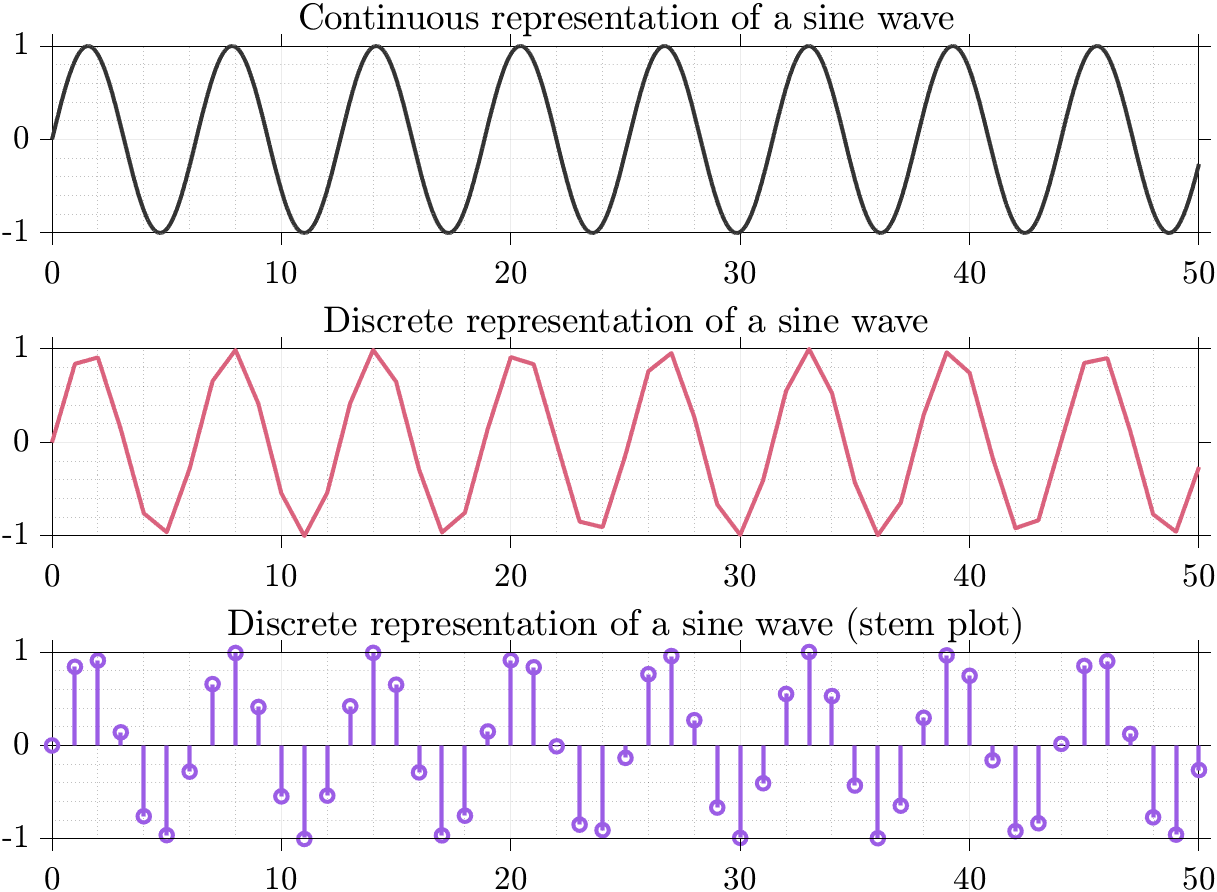
\includegraphics[width=0.45\linewidth, trim=0 0 0 0cm,clip]{figures/sampled_sine_wave.png} 
    
    $x[n] = x(nT_s)$,
$T_s$ = sample time.
    
    \tiny
    Code for the figure: \url{https://github.com/rahulbhadani/CPE381_FA25/blob/main/Code/sampled_sine_wave.m}
\end{frame}

\begin{frame}{Sampling Process}
    \begin{itemize}
        \item \( x[n] = x(nT_s) = x(t)|_{t=nT_s} \)
        \item This equation represents the \textbf{sampling process} where a continuous-time signal \( x(t) \) is sampled at uniform intervals \( T_s \) to produce a discrete-time signal \( x[n] \).
        \item \textbf{Key Points:}
            \begin{itemize}
                \item \( n \) is an integer representing the sample index.
                \item \( T_s \) is the sampling period.
                \item The continuous-time signal \( x(t) \) is sampled at \( t = nT_s \).
            \end{itemize}
    \end{itemize}
\end{frame}

\begin{frame}
\frametitle{Derivatives and Finite Differences}
\textbf{Continuous-Time Derivatives:}
\begin{itemize}
    \item Derivatives measure the rate of change of a function.
    \item Defined as the limit of the difference quotient as the interval approaches zero.
    \item Represented as \( \frac{dy}{dt} \) for a function \( y(t) \).
\end{itemize}
\end{frame}

\begin{frame}
\frametitle{Finite Differences}
\textbf{Discrete-Time Derivatives:}
\begin{itemize}
    \item Finite differences approximate derivatives for discrete-time signals.
    \item Forward difference: \( \Delta x[n] = x[n+1] - x[n] \).
    \item Backward difference: \( \Delta x[n] = x[n] - x[n-1] \).
\end{itemize}
\vspace{5pt}
$x[n] = x(nT_s)$ when looking at continuous to discrete domain where $T_s$ is the sampling time, $n$ is any positive integer. We will look at this much later in detail.
\end{frame}

\begin{frame}
\frametitle{Central Differences}
\textbf{Central Difference:}
\begin{itemize}
    \item Provides a more accurate approximation.
    \item Defined as \( \delta x[n] = \frac{x[n+1] - x[n-1]}{2} \).
    \item Reduces error compared to forward and backward differences.
\end{itemize}
\end{frame}


\begin{frame}{Relation between the Derivative and Finite Difference}
    The derivative and the finite-difference operators are not the same. In the limit, we have:
    \begin{equation*}
            \frac{dx(t)}{dt}|_{t = nT_s} = \lim_{T_s\to 0 }\cfrac{\Delta [x (nT_s)]}{T_s}
    \end{equation*}

\end{frame}

\begin{frame}
\frametitle{Applications}
\textbf{Applications of Finite Differences:}
\begin{itemize}
    \item Used in numerical methods for solving differential equations.
    \item Essential in digital signal processing and control systems.
    \item Helps in approximating continuous-time derivatives in discrete systems.
\end{itemize}
\end{frame}

\begin{frame}{Discrete Integration}
Recall, the integration in the continuous domain is 
$$
I(t) = \int_{t_0}^t x(\tau) d\tau
$$
then, we have 
$$
\cfrac{d}{dt} \int_{t_0}^t x(\tau) d\tau = x(t)
$$

If we use $D$ for the derivative operator, then $D^{-1}$ is the integration operator.

$$
D[ D^{-1}[x(t)]] = x(t))
$$
\end{frame}

\begin{frame}
\frametitle{Example}
\begin{columns}
\column{0.5\linewidth}
    \begin{itemize}
    \item Computational integration using sums:
    $$
    \int_{0}^{10} t \, dt = \frac{t^2}{2} \bigg|_{0}^{10} = 50
    $$
\end{itemize}
\column{0.5\linewidth}
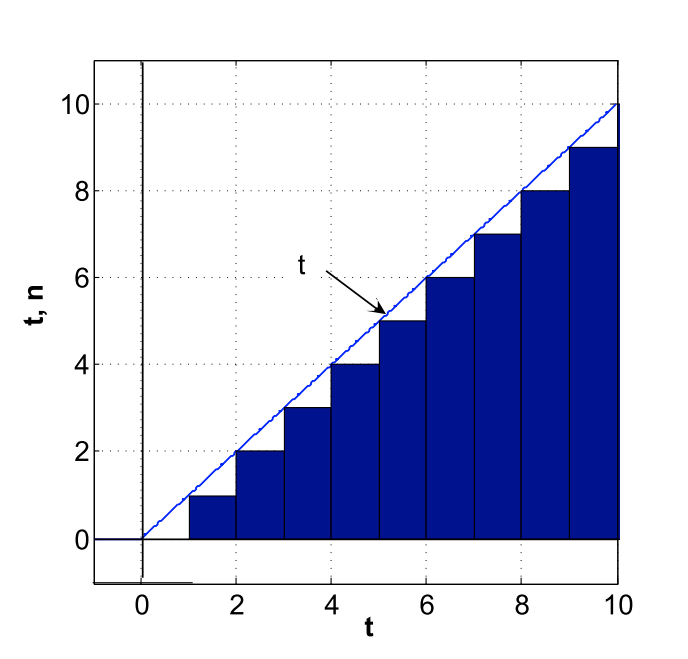
\includegraphics[width=0.7\linewidth, trim=0 0 0 0cm,clip]{figures/slopeline.png} 
\end{columns}

\end{frame}

\begin{frame}
\frametitle{Discrete Approximation}
\begin{columns}
\column{0.5\linewidth}
\begin{itemize}
    \item Approximation using pulses ($T_s = 1$)(rectangle of width $T_s = 1$, height = $n$):
    $$
    \sum_{n=0}^{9} p[n] = \sum_{n=0}^{9} n = 45
    $$
    \item Generalized sum:
    $$
    \sum_{n=0}^{N-1} n = \frac{N \times (N-1)}{2}
    $$
\end{itemize}
\column{0.5\linewidth}
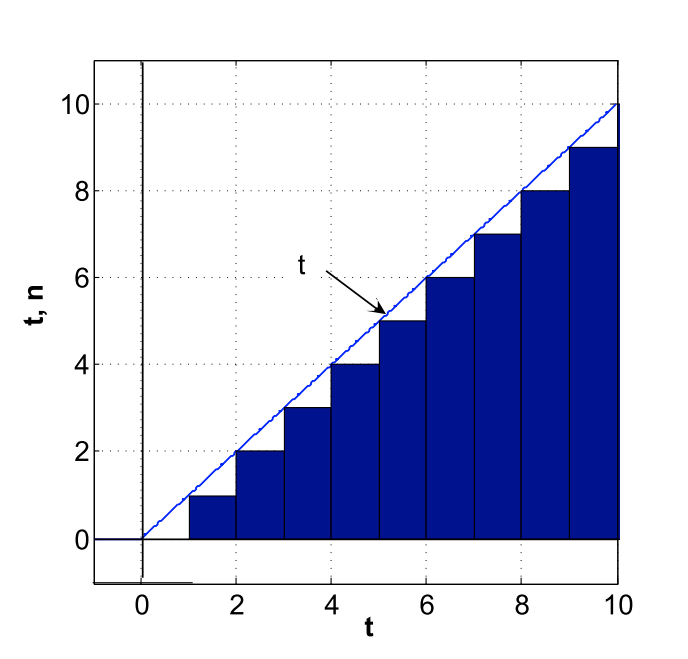
\includegraphics[width=0.7\linewidth, trim=0 0 0 0cm,clip]{figures/slopeline.png} 
\end{columns}


\end{frame}

\begin{frame}
\frametitle{Improved Discrete Approximation}
\begin{itemize}
    \item Using \( T_s = 10^{-3} \):
    $$
    \sum_{n=0}^{(10/T_s)-1} nT_s^2 = \sum_{n=0}^{(10/T_s)-1} n 10^{-6} = = 49.995
    $$
    The height of each pulse is $nT_s$ and the width is $T_s$.
\end{itemize}

Hence, the sampling time (or its inverse -- sampling frequency matters).
\end{frame}

\begin{frame}{Solving Ordinary Differential Equations using Numerical Methods}
Recognizing that derivatives can be approximated as difference equations in the discrete domain, we have some methods to solve ordinary differential equations, suitable for computer implementations.

Some common numerical methods to solve ODE are:
\begin{itemize}
    \item Euler's Method
    \item Runge-Kutta Method (4th Order)
\end{itemize}
\end{frame}

\begin{frame}
\frametitle{Euler's Method}
\begin{itemize}
    \item Consider the ODE: $ \frac{dy}{dt} = f(t, y) $
    \item Initial condition: $ y(t_0) = y_0 $
    \item Euler's method formula: $ y_{n+1} = y_n + h f(t_n, y_n) $
    \item Example: $ \frac{dy}{dt} = -2y, \quad y(0) = 1 $
    \item Using $ h = 0.1 $: $ y_{n+1} = y_n - 0.2y_n = y_n(1 - 0.2) $
\end{itemize}
\end{frame}

\begin{frame}
  \frametitle{Euler's Method}
  \textbf{Euler's method:}
  \begin{equation*}
    y_{n+1} = y_n + hf(t_n, y_n)
  \end{equation*}
  
  \textbf{Example:} Solve $y' = 2t$ with $y(0) = 1$ using Euler's method with $h = 0.1$
  \begin{itemize}
    \item In this case, $f(t, y) = 2t$
  \end{itemize}
  \begin{table}
    \begin{tabular}{c|c|c}
      $t_n$ & $y_n$ & $y_{n+1}$ \\
      \hline
      0 & 1 & 1.0 \\
      0.1 & 1.0 & 1.02 \\
      0.2 & 1.02 & 1.06 \\
      \vdots & \vdots & \vdots
    \end{tabular}
  \end{table}
\end{frame}

\begin{frame}
\frametitle{Runge-Kutta Method (4th Order)}
\begin{columns}
    \column{0.5\linewidth}
    \begin{itemize}
          \item Consider the ODE: $ \frac{dy}{dt} = f(t, y) $
    \item Initial condition: $ y(t_0) = y_0 $
    \item Runge-Kutta method formula:
    $$
    \begin{aligned}
    k_1 &= h f(t_n, y_n) \\
    k_2 &= h f\left(t_n + \frac{h}{2}, y_n + h \frac{k_1}{2}\right) \\
    k_3 &= h f\left(t_n + \frac{h}{2}, y_n + h \frac{k_2}{2}\right) \\
    k_4 &= h f(t_n + h, y_n + h k_3) \\
    y_{n+1} &= y_n + \frac{1}{6}(k_1 + 2k_2 + 2k_3 + k_4)
    \end{aligned}
    $$
    \end{itemize}

\column{0.5\linewidth}
\begin{itemize}
  
    \item Example: $ \frac{dy}{dt} = t + y, \quad y(0) = 1 $
    \item Using $ h = 0.1 $:
   
    Write a MATLAB code to implement that.
\end{itemize}
\end{columns}
\end{frame}



\begin{frame}
  \frametitle{Runge-Kutta Methods}
  \textbf{Runge-Kutta methods:}
  \begin{itemize}
    \item More accurate than Euler's method
    \item Use multiple function evaluations at each step
  \end{itemize}
  \textbf{Example:} Solve $y' = 2x$ with $y(0) = 1$ using the Runge-Kutta method of order 4 with $h = 0.1$
  \begin{table}
    \begin{tabular}{c|c|c}
      $x_n$ & $y_n$ & $y_{n+1}$ \\
      \hline
      \vdots & \vdots & \vdots
    \end{tabular}
  \end{table}
\end{frame}

\section{Numerical Computation in MATLAB}

\begin{frame}{}
    \begin{center}
    \Huge \bf \color{DarkBlue}
    \faFire
    
Numerical Computation in MATLAB

\end{center}
\end{frame}


\begin{frame}[containsverbatim]{Differentiation in MATLAB}
    $$
    y(t) = \cos(t^2)
    $$
\end{frame}
\begin{frame}[containsverbatim]{Differentiation in MATLAB}
    \footnotesize
\begin{columns}
    \column{0.5\linewidth}
    \begin{verbatim}
%% Solving derivatives symbolically
% y(t) = cos(t^2)
% dy/dt = -2*t*sin(t^2)
%% Symbolic derivative: the ground truth
syms t y z % we define symbols
y = cos(t^2);
z = diff(y);
figure(1);
subplot(2, 1, 1)
% symbolic plotting
fplot(y, [0, 2*pi], 'LineWidth', 3);
grid on;
hold on;
subplot(2, 1, 2);
fplot(z, [0, 2*pi], 'LineWidth', 3);
grid on;
hold on;
    \end{verbatim}
    \column{0.5\linewidth}
    \begin{verbatim}
%% Numerical derivative
Ts = 0.1;
t1 = 0:Ts:2*pi;
y1 = cos(t1.^2);
z1 = diff(y1)./diff(t1);
figure(1);
subplot(2, 1, 1);
stem(t1, y1, 'r');
subplot(2, 1, 2);
stem(t1(1:length(y1) -1), z1, 'm' );

    \end{verbatim}
\end{columns}
\end{frame}

\begin{frame}{Integration in MATLAB}

\footnotesize
    $$
    \int\cfrac{x^3}{x+2} dx
    $$

    \begin{multiequation}
  \int\frac{x^3}{x+2} dx &= \int\frac{x^3+8-8}{x+2} dx & \text{Add and subtract 8 to the numerator} \\
  &= \int\frac{(x+2)(x^2-2x+4)-8}{x+2} dx & \text{Factor the numerator} \\
  &= \int\left(x^2-2x+4-\frac{8}{x+2}\right) dx & \text{Split the fraction} \\
  &= \int x^2 dx - 2\int x dx + 4\int dx - 8\int\frac{1}{x+2} dx & \text{Split the integral into separate terms} \\
  &= \frac{x^3}{3} - x^2 + 4x - 8\ln|x+2| + C & \text{Evaluate each integral}
\end{multiequation}
\end{frame}

\begin{frame}[containsverbatim]{Integration in MATLAB}
    \small
    \begin{columns}
    \column{0.4\linewidth}
    \begin{verbatim}
%% Symbolic Integration
% x^3/(x + 2) dx
syms x
f = x^3/(x + 2)
% indefinite integral
int(f)
% definite integral
int(f, 0, 10)
    \end{verbatim}
    \column{0.6\linewidth}
    \begin{verbatim}
%% Numerical Integration using trapezoidal rule, 
%% Numerical integration is always definite
x = 0:0.1:10;
f = x.^3./(x + 2);
trapz(x, f)
    \end{verbatim}
\end{columns}
\end{frame}


\begin{frame}{Ordinary Differential Equation in MATLAB}
Solve the initial value problem $ty' + 3y = 0, y(1) = 2$, assuming $t > 0$. We write the equation in standard form: $y' + 3y/t = 0$.

$$
P(t) = \int -\cfrac{3}{t}dt  = -3 \ln t
$$

and


$$
y = Ae^{-3\ln t} = At^{-3}
$$
Substitute to find $A$: $ 2= A(1)^{-3}$, so the solution is $y = 2t^{-3}$.
    
\end{frame}


\begin{frame}[containsverbatim]{Ordinary Differential Equation in MATLAB}
    \small
    \begin{verbatim}
%% ty; + 3y = 0; y(1) = 2
% solution y = 2/t^3
syms y(t)
eqn = diff(y, t) + 3*y/t ==0;
cond = y(1) == 2;
y(t) = dsolve(eqn, cond);
    \end{verbatim}
\end{frame}
\end{document}